We know that,
\begin{align}
\int_{-\infty}^{\infty}{f_x(x)}\,dx = 1.\\
\int_{-\infty}^{0}{f_x(x)}\,dx +\int_{0}^{\infty}{f_x(x)}\,dx = 1\label{ee2016-33:eq_(1)}\\
\int_{-\infty}^{0}{ae^{4x}}\,dx +\int_{0}^{\infty}{\frac{3}{2}e^{-3x}}\,dx = 1\label{ee2016-33:eq_(2)}
\end{align}
The expression \eqref{ee2016-33:eq_(2)} was written from \eqref{ee2016-33:eq_(1)} since,
\begin{align*}
  u(x) = 
  \begin{cases}
  1, & \text{for } x \geq 0\\
  0, & \text{otherwise } 
  \end{cases}
\end{align*}

Simplifying \eqref{ee2016-33:eq_(2)} we have:
\begin{align}
\int_{-\infty}^{0}{ae^{4x}}\,dx +\int_{0}^{\infty}{\frac{3}{2}e^{-3x}}\,dx = 1\nonumber\\
\implies a\left[\frac{e^{4x}}{4}\right]_{-\infty}^{0} +    \frac{3}{2}\left[\frac{e^{-3x}}{-3}\right]_0^{\infty} = 1\\
\implies a\left[\frac{1}{4}-0\right] - \frac{1}{2}\left[0-1\right] = 1\\
\implies \frac{a}{4} + \frac{1}{2} =1 \implies a = 2
\end{align}
Therefore,
\begin{align}
 f_x(x) = 
  \begin{cases}
  \frac{3}{2}e^{-3x}, & \text{for } x \geq 0\\
  2e^{4x}, & \text{for } x < 0
  \end{cases}
\end{align}

The plot for PDF of $X$ can be observed at figure \ref{ee2016-33:fig:The PDF of X}
\begin{figure}[!ht]
       \centering
    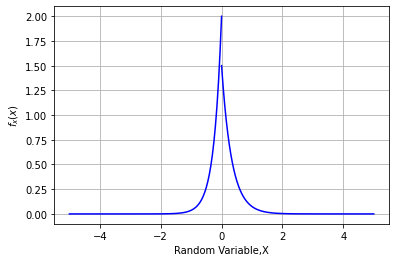
\includegraphics[width=.9\columnwidth] {solutions/ee/2016/33/Assignment_2_Fig_2.png}
    \caption{The PDF of X}
    \label{ee2016-33:fig:The PDF of X}
\end{figure}

The CDF of X is defined as follows:
\begin{align}
    F_X(x)= \pr{X\leq x}
\end{align}
Now for $x<0$,
\begin{align}
\pr{X\leq x} &= \int_{-\infty}^{x}{f_x(x)}\,dx\\
&= \int_{-\infty}^{x}{2e^{4x}}\,dx\\
&= 2\left[\frac{e^{4x}}{4}\right]_{-\infty}^{x}\\
&= 2\left[\frac{e^{4x}}{4}-0\right]\\
&= \frac{e^{4x}}{2}
\end{align}
Similarly for $x\geq0$,
\begin{align}
\pr{X\leq x} &= \int_{-\infty}^{x}{f_x(x)}\,dx\\
&= \int_{-\infty}^{0}{2e^{4x}}\,dx +\int_{0}^{x}{\frac{3}{2}e^{-3x}}\,dx\\
&= 2\left[\frac{e^{4x}}{4}\right]_{-\infty}^{0}+\left[\frac{-e^{-3x}}{2}\right]_{0}^{x}\\
&= 2\left[\frac{1}{4}-0\right]-\frac{1}{2}\left[e^{-3x}-1\right]\\
&= 1-\frac{e^{-3x}}{2}
\end{align}

The CDF of X is as below:
\begin{align}
 F_X(x) = 
  \begin{cases}
  1-\frac{e^{-3x}}{2}, & \text{for } x \geq 0\\
  \frac{e^{4x}}{2}, & \text{for } x < 0
  \end{cases}
\end{align}

The plot for CDF of $X$ can be observed at figure \ref{ee2016-33:fig:The PDF of X}.
\begin{figure}[!ht]
       \centering
    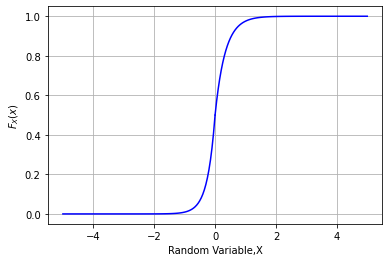
\includegraphics[width=.9\columnwidth] {solutions/ee/2016/33/Assignment_2_Fig_1.png}
    \caption{The CDF of X}
    \label{ee2016-33:fig:The CDF of X}
\end{figure}

\begin{align}
\therefore
\pr{X\leq0} = F_X(0)=\frac{1}{2}
\end{align}


